\chapter{Описание экспериментов и анализ} \label{ch:ch3}

\section{Рассмотренные алгоритмы}

\noindent В текущей работе были рассмотрены следующие алгоритмы:

\begin{enumerate}
	\item k-Nearest Neighbors (k-NN) \cite{knn} -- метод k-ближайших соседей.
	\item Principal Component Analysis (PCA) \cite{pca} -- метод главных компонент.
	\item One-Class Support Vector Machines (OCSVM) \cite{ocsvm} -- одноклассовый метод опорных векторов.
	\item Local Outlier Factor (LOF) \cite{lof} -- метод локального уровеня выброса.
	\item Histogram-Based Outlier Score (HBOS) \cite{hbos} -- оценка выбросов на основе гистограммы.
	\item Isolation Forest (IFOREST) \cite{iforest} -- метод изолируещего леса.
\end{enumerate}

\subsection{k-Nearest Neighbors (k-NN)}

Алгоритм для автоматической классификации объектов. Каждый объект выборки относится к тому классу, который является наиболее распространённым среди $k$ соседей рассматриваемого объекта, классы которых уже известны. Алгоритм может быть применим к многомерным наборам данных -- в таком случае перед применением необходимо определить функцию расстояния (метрику). Классический вариантом такой функции является евклидово расстояние. На~рисунке~\ref{fig:knn} приведён пример классификации методом k-ближайших соседей.

\begin{figure}[ht]
  \centering
  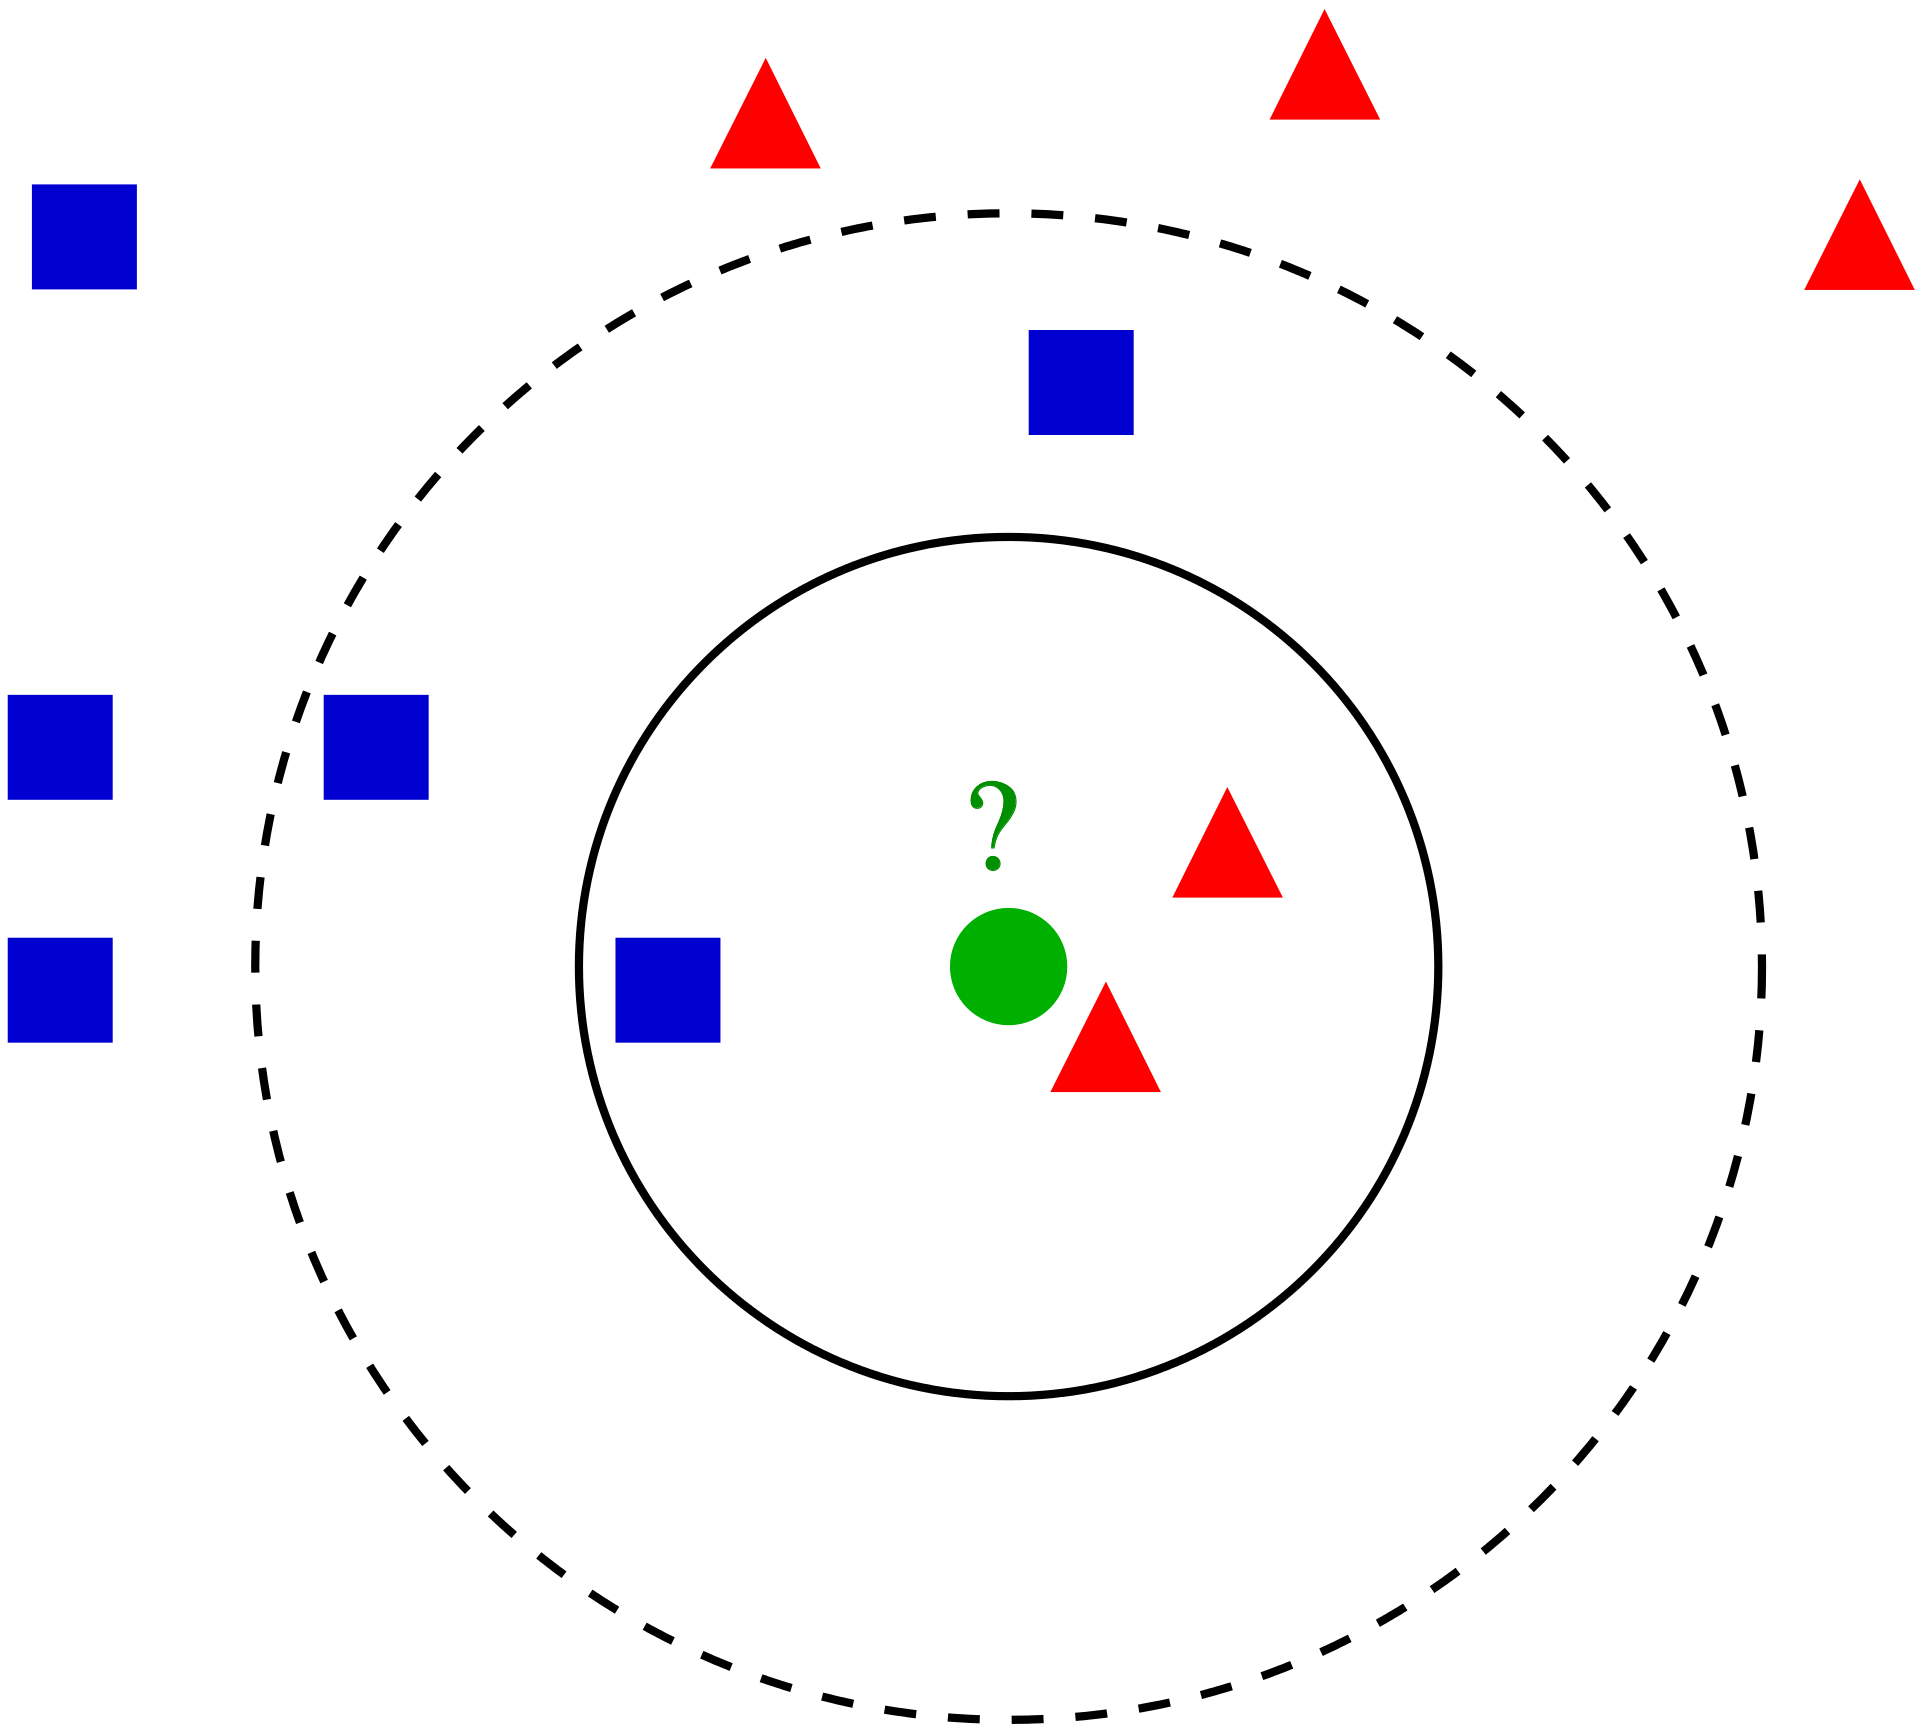
\includegraphics [scale=0.1] {knn}
  \caption{Тестовый образец (зелёный круг) должен быть классифицирован как синий квадрат (класс 1) или как красный треугольник (класс 2). Если $k = 3$, то он классифицируется как класс 2, потому что внутри меньшего круга 2 треугольника и только 1 квадрат. Если $k = 5$, то он будет классифицирован как класс 1 (3 квадрата против 2 треугольников внутри большего круга).}
  \label{fig:knn}
\end{figure}

\subsection{Principal Component Analysis (PCA)}

Название алгоритма переводится как "метод главных компонент". Он применяется во многих областях, в том числе, биоинформатике, обработке изображений, для сжатия данных, в общественных науках. Вычисление этих главных компонент может быть сведено к вычислению сингулярного разложения матрицы данных или к вычислению собственных векторов и собственных значений ковариационной матрицы исходных данных. На~рисунке~\ref{fig:pca} представлены собственные векторы в случае двумерной гауссианы.

\begin{figure}[ht]
  \centering
  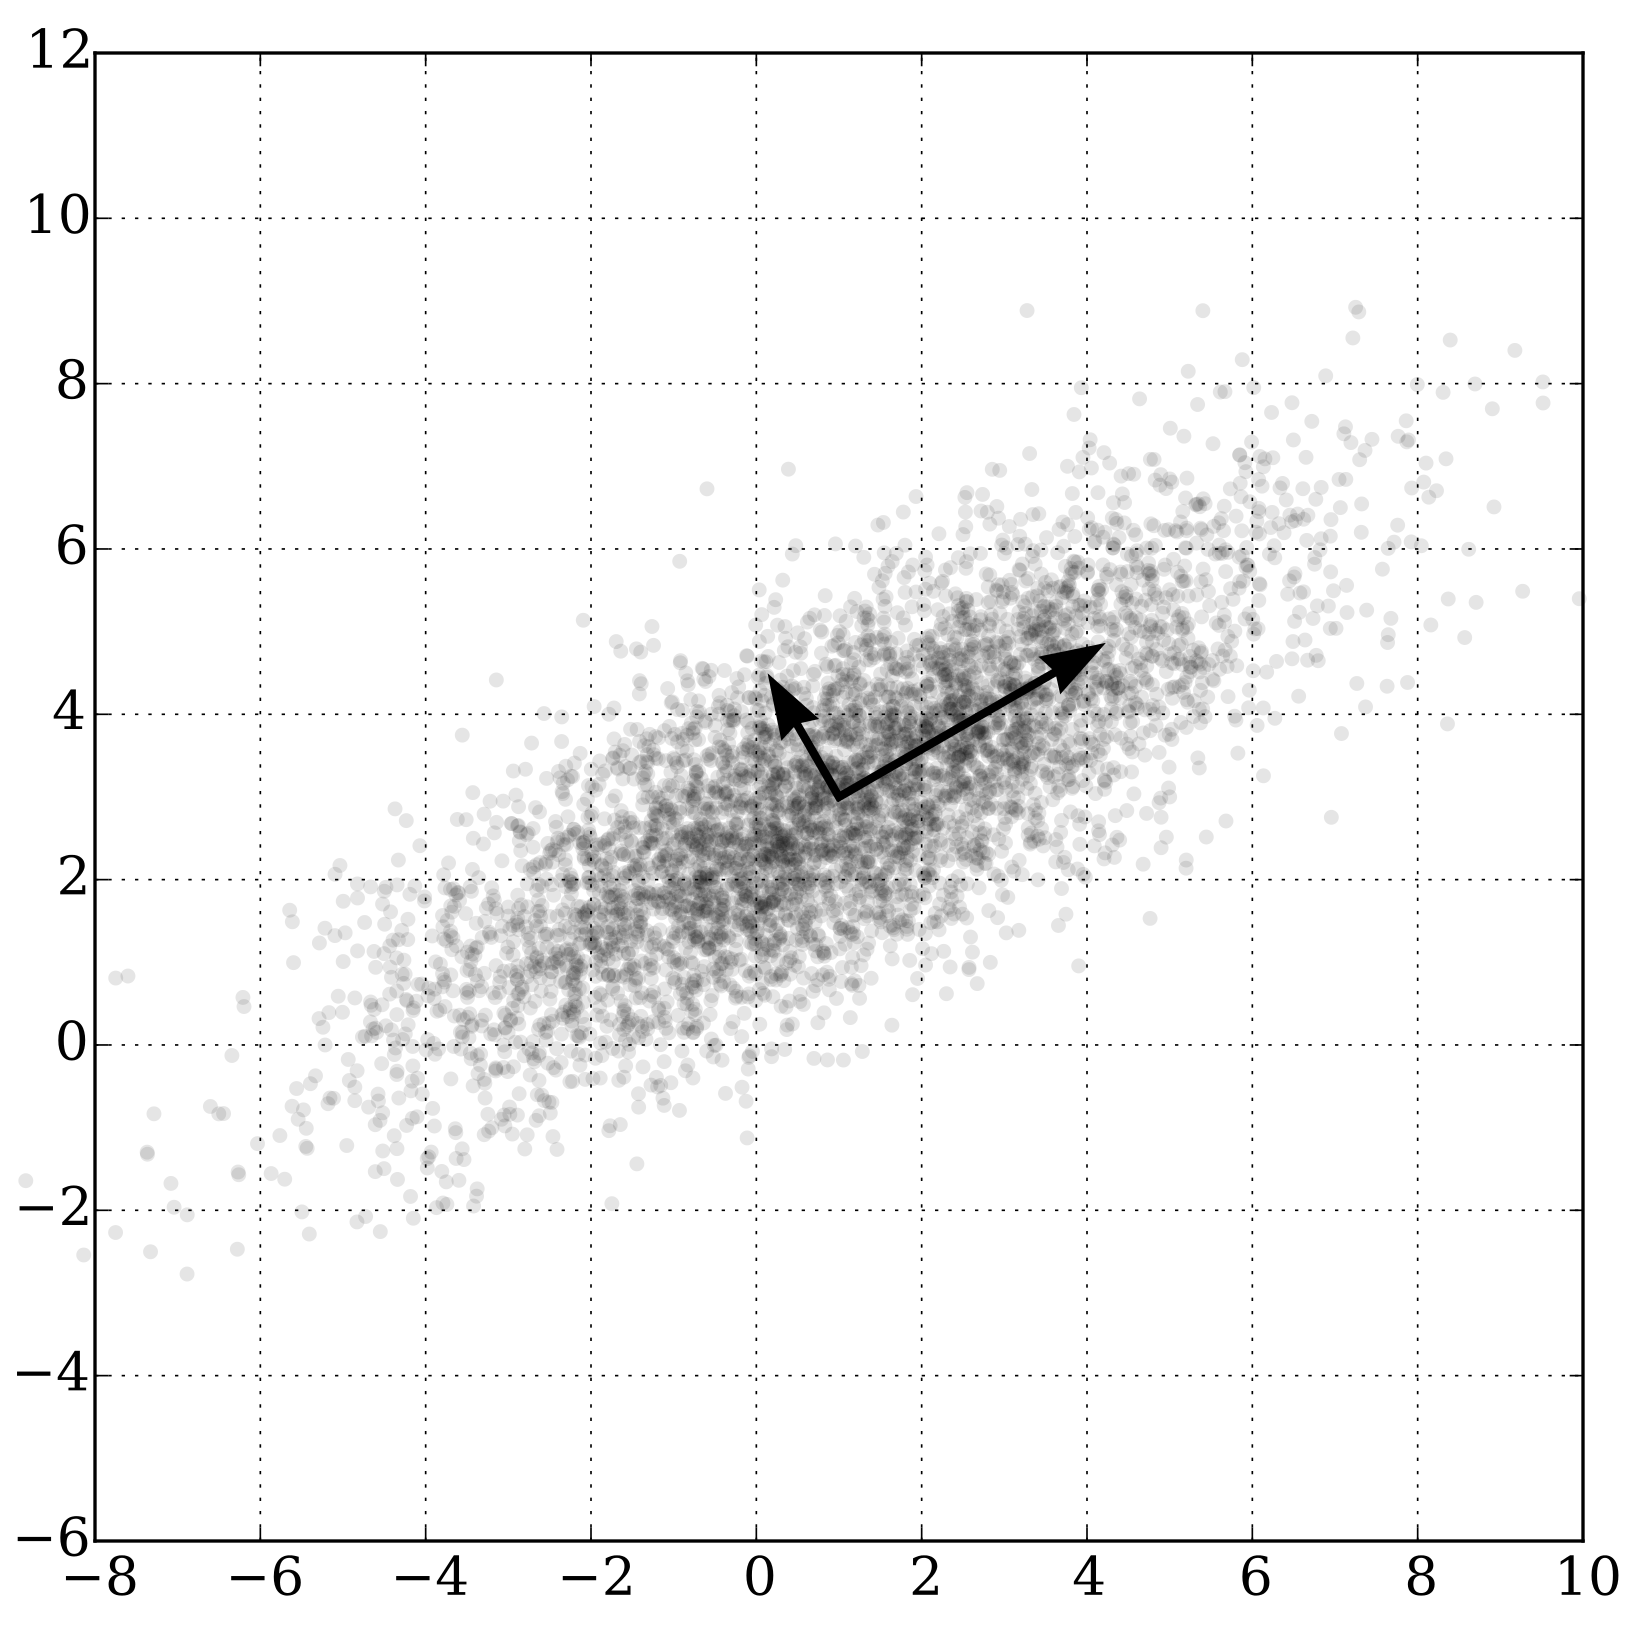
\includegraphics [scale=0.15] {pca}
  \caption{PCA для многомерного гауссового распределения с центром в точке (1, 3) со стандартным отклонением 3. Векторы отражают собственные векторы ковариационной матрицы гауссианы.}
  \label{fig:pca}
\end{figure}

\subsection{One-Class Support Vector Machines (OCSVM)}

В русской литературе алгоритм часто называют "методом опорных векторов". Он относится к семейству линейных классификаторов. Особым свойством метода опорных векторов является непрерывное уменьшение эмпирической ошибки классификации и увеличение зазора, поэтому метод также известен как метод классификатора с максимальным зазором.

Основная идея метода -- перевод исходных векторов в пространство более высокой размерности и поиск разделяющей гиперплоскости с максимальным зазором в этом пространстве. Две параллельных гиперплоскости строятся по обеим сторонам гиперплоскости, разделяющей классы. Разделяющей гиперплоскостью будет гиперплоскость, максимизирующая расстояние до двух параллельных гиперплоскостей. На~рисунке~\ref{fig:svm} продемонстрирована работа алгоритма.

\begin{figure}[ht]
  \centering
  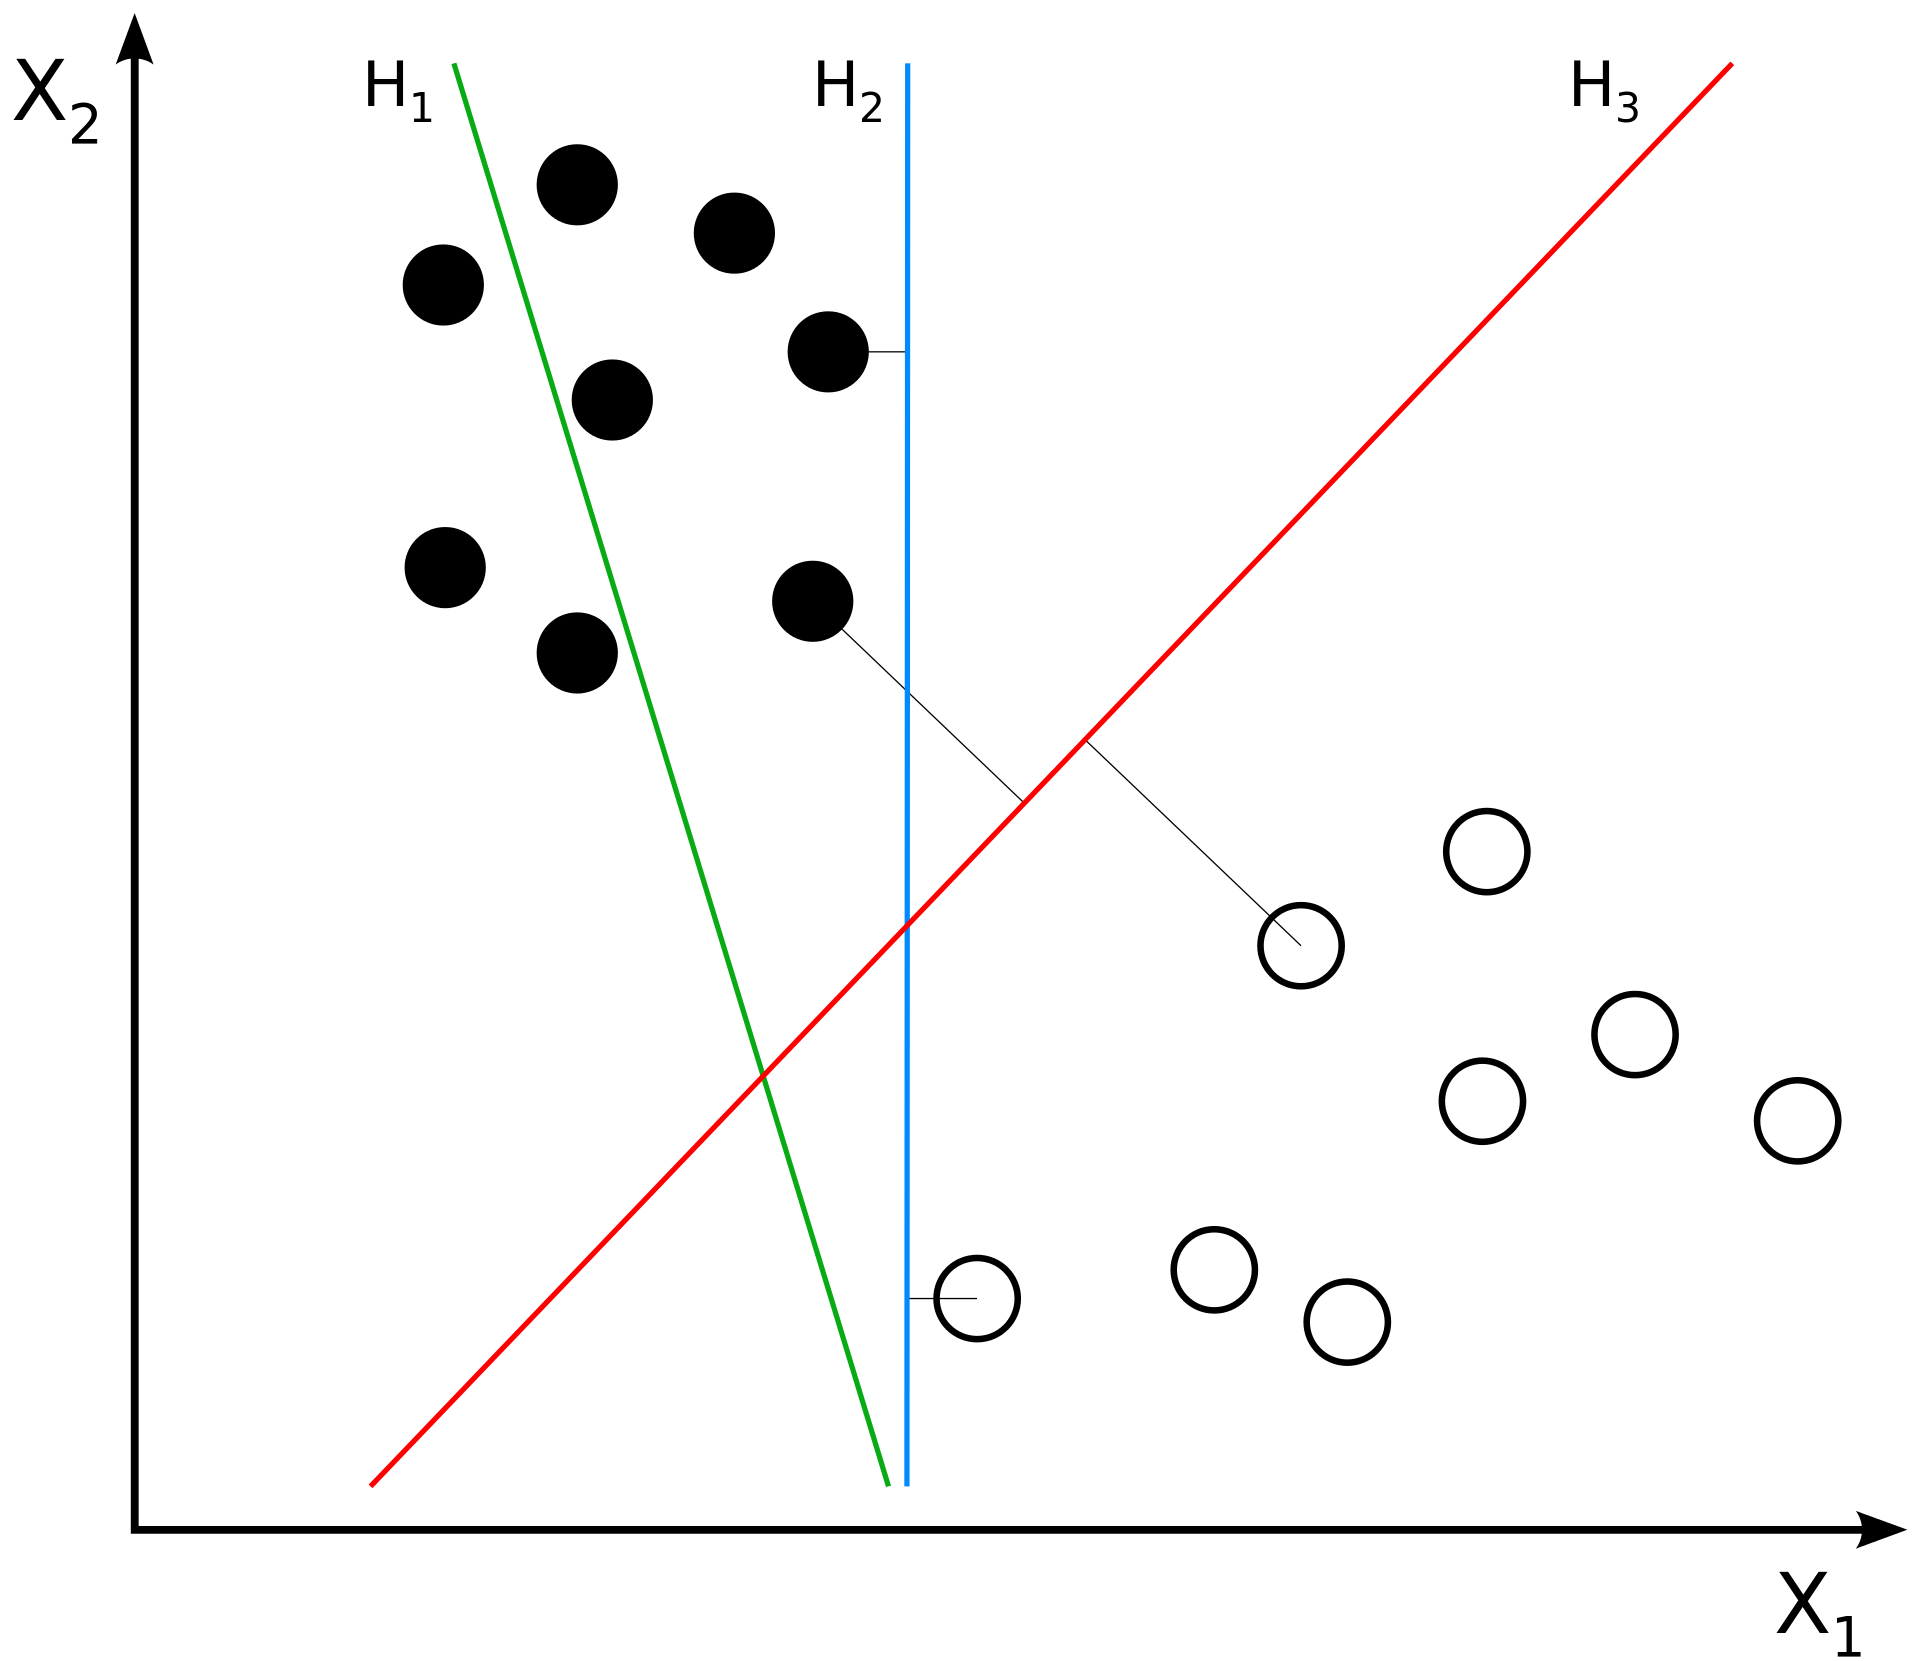
\includegraphics [scale=0.1] {svm}
  \caption{Гиперплоскость $H1$ не разделяет классы. В случае гиперплоскости $H2$ разделение имеется, но зазор слишком маленький. Разделение с максимальным зазором достигается гиперплоскостью $H3$.}
  \label{fig:svm}
\end{figure}

\subsection{Local Outlier Factor (LOF)}

Локальный уровень выброса основывается на концепции локальной плотности, где локальность задаётся $k$ ближайшими соседями, расстояния до которых используются для оценки плотности. Путём сравнения локальной плотности объекта с локальной плотностью его соседей, можно выделить области с аналогичной плотностью и точки, которые имеют существенно меньшую плотность, чем её соседи. Эти точки считаются аномалиями.

Локальная плотность оценивается расстоянием, с которым точка может быть "достигнута" от соседних точек. Определение "расстояния достижимости", используемого в алгоритме, является дополнительной мерой для получения более устойчивых результатов внутри кластеров. На~рисунке~\ref{fig:lof} разобрана базовая идея алгоритма.

\begin{figure}[ht]
  \centering
  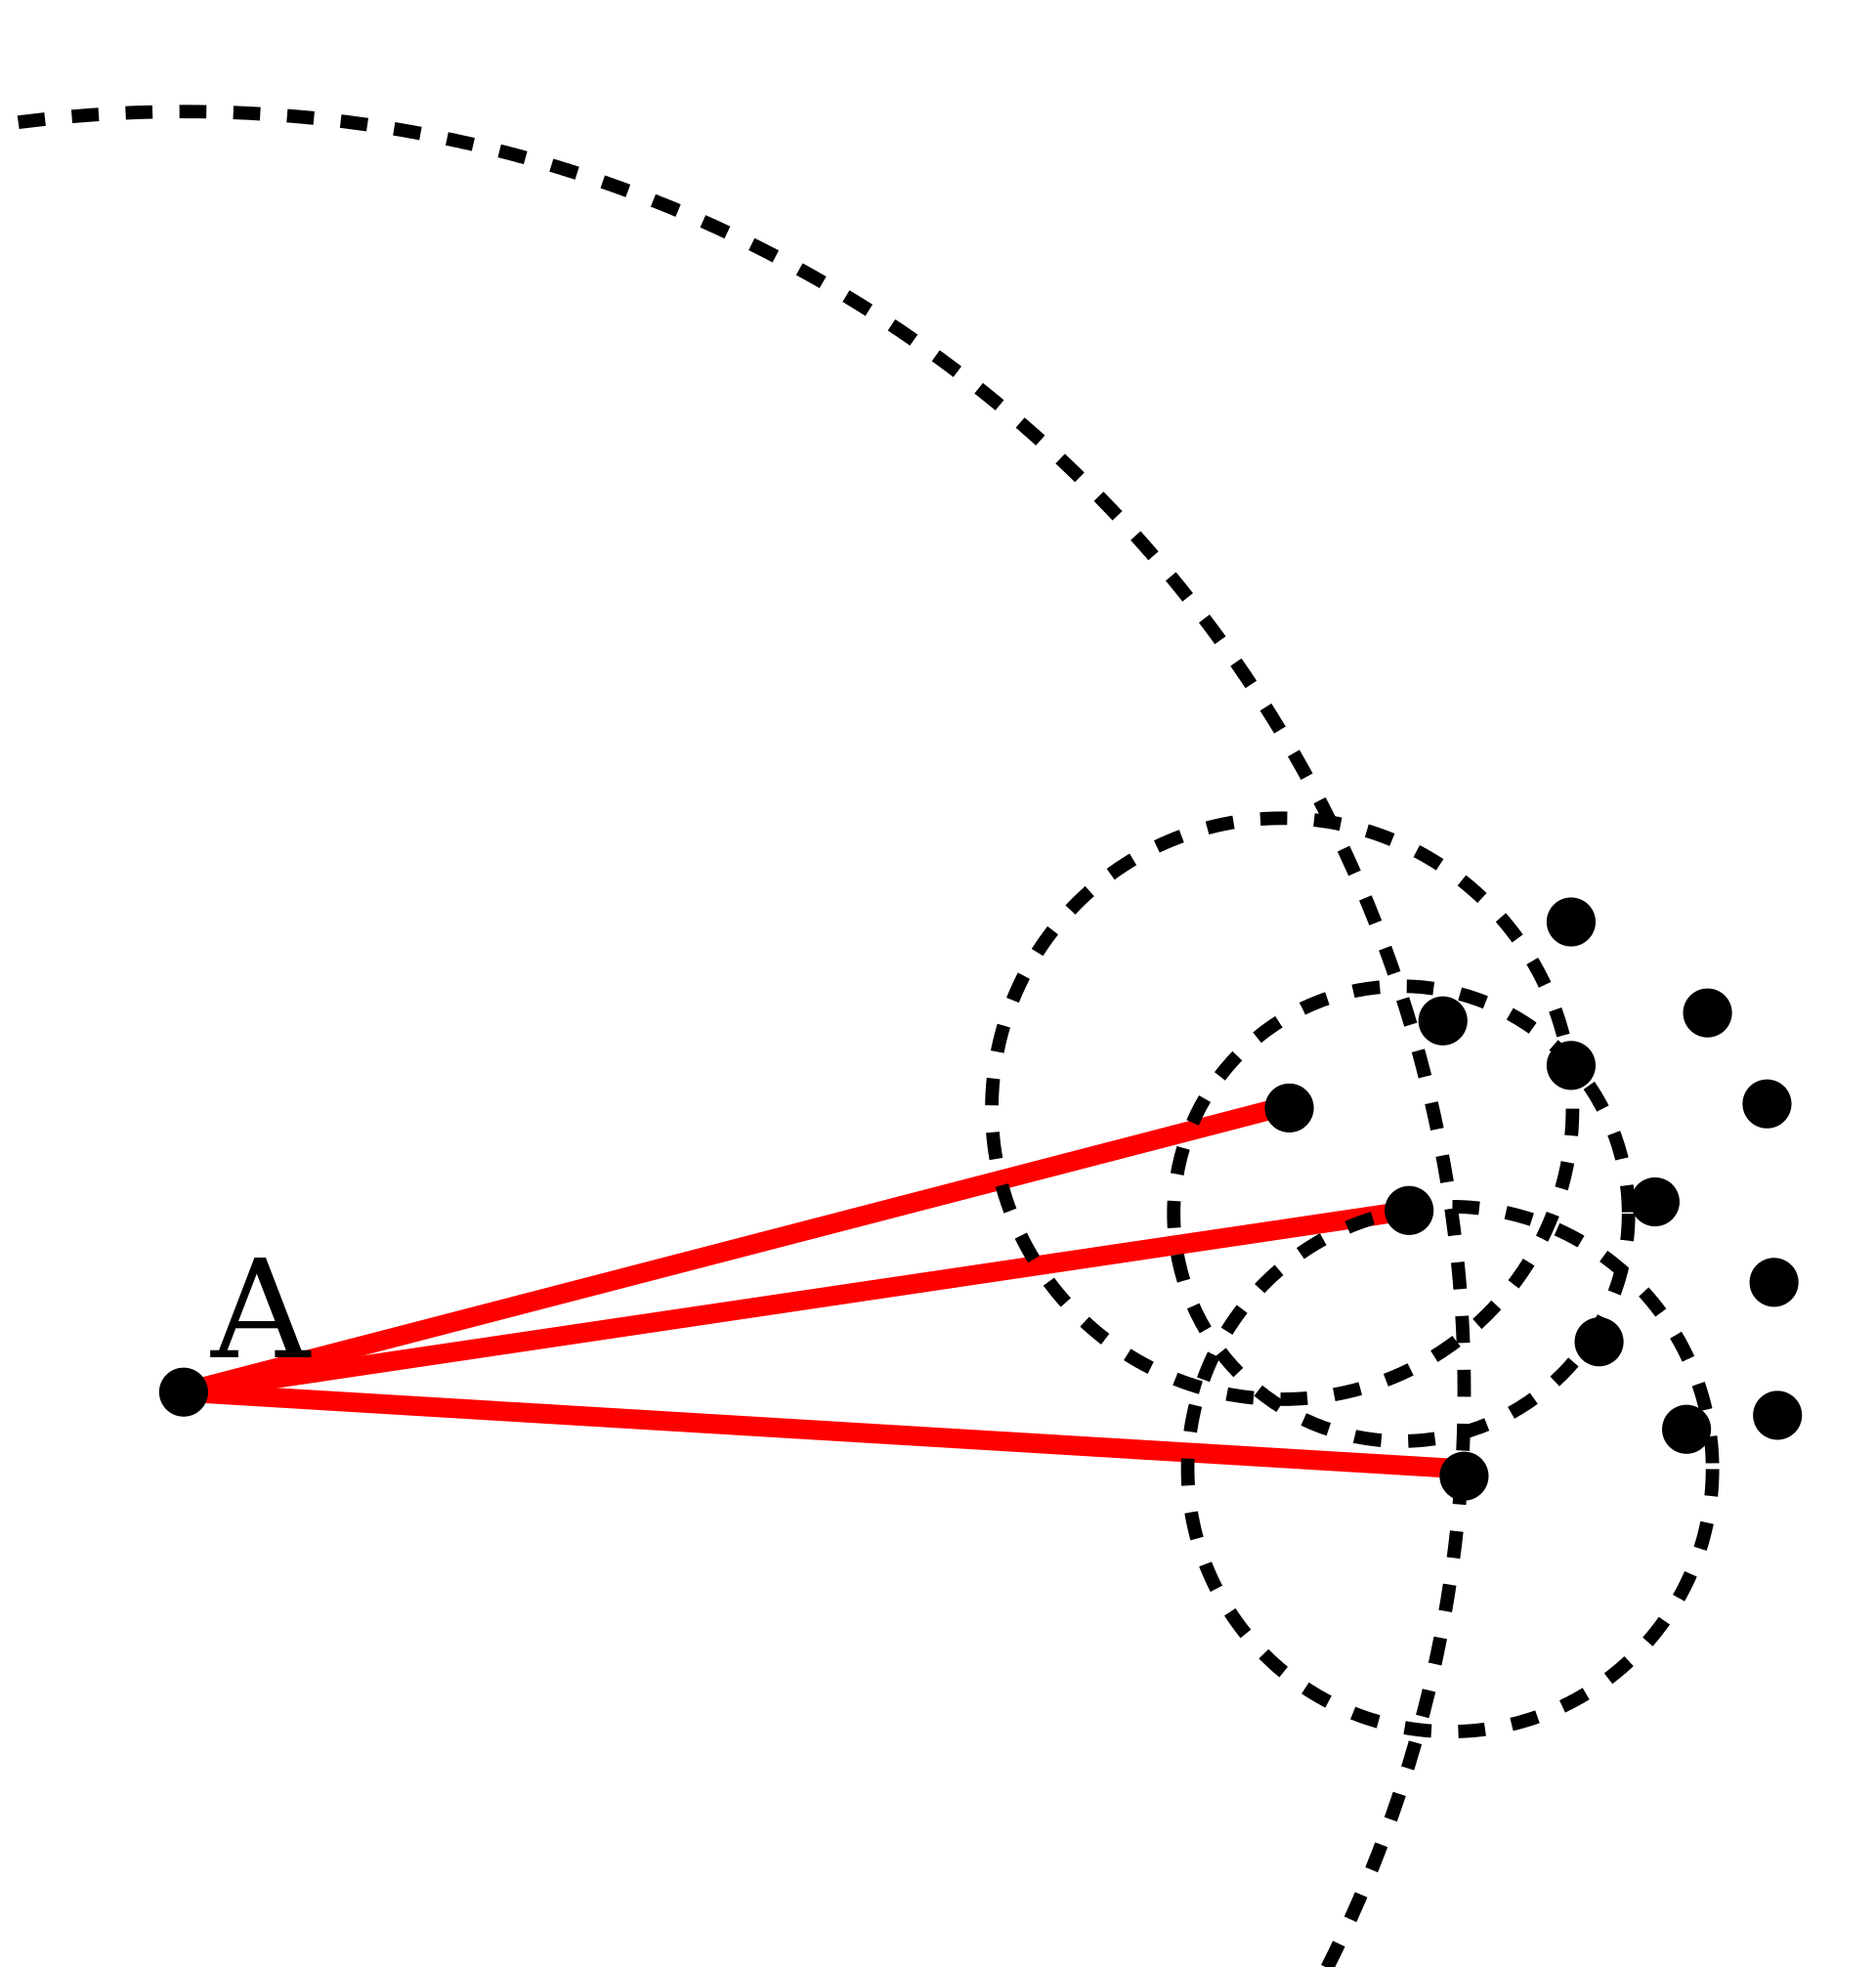
\includegraphics [scale=0.1] {lof}
  \caption{Базовая идея метода -- сравнение локальной плотности точки с плотностями её соседей. Точка A имеет меньшую плотность по сравнению с соседями}
  \label{fig:lof}
\end{figure}

\subsection{Histogram-Based Outlier Score (HBOS)}

Алгоритм HBOS в несколько раз быстрее работает, чем алгоритмы, основанные на кластеризации и методе ближайших соседей. Для каждого измерения $d$ строится одномерная гистограмма, где высота каждой ячейки отражает оценку плотности. Затем проводится нормировка таким образом, что максимальная высота ячеек каждой гистограммы составляет $1.0$. Это обеспечивает равный вклад каждого измерения в оценку аномальности. Наконец, для каждого объекта $p$ выборки рассчитывается $HBOS$, используя высоту соответствующей ячейки, в которой объект расположен:

\[HBOS\left(p\right) = \sum_{i=0}^{d}\log\left(\frac{1}{hist_i\left(p\right)}\right).\]

Вместо произведения используется сумма логарифмов -- это то же самое, что и применение логарифма к произведению $\left(\log\left(a\cdot b\right) = \log\left(a\right)+\log\left(b\right)\right)$. Такой подход менее чувствительный к ошибкам, которые связаны с точностью плавающей точки в экстремально несбалансированных распределениях, что в свою очередь может приводить к очень высоким значениям оценки аномальности. Подробнее про алгоритм можно найти информацию в \cite{hbos}.

\subsection{Isolation Forest (IFOREST)}

Один из вариантов случайного леса (строится из решающих деревьев). Выбирается случайный признак и случайное разделение, по которым строится ветвление в дереве. Для каждого объекта выборки определяется мера его нормальности как среднее арифметическое глубин листьев, в которые он попал (под этим понимается "изоляция").

При таком способе построения деревьев аномалии будут попадать в листья на ранних этапах (на небольшой глубине дерева), то есть выбросы проще "изолировать". Дерево строится до тех пор, пока каждый объект не окажется в отдельном листе). На~рисунке~\ref{fig:iforest} продемонстрирована основная идея метода.

\begin{figure}[ht]
  \centering
  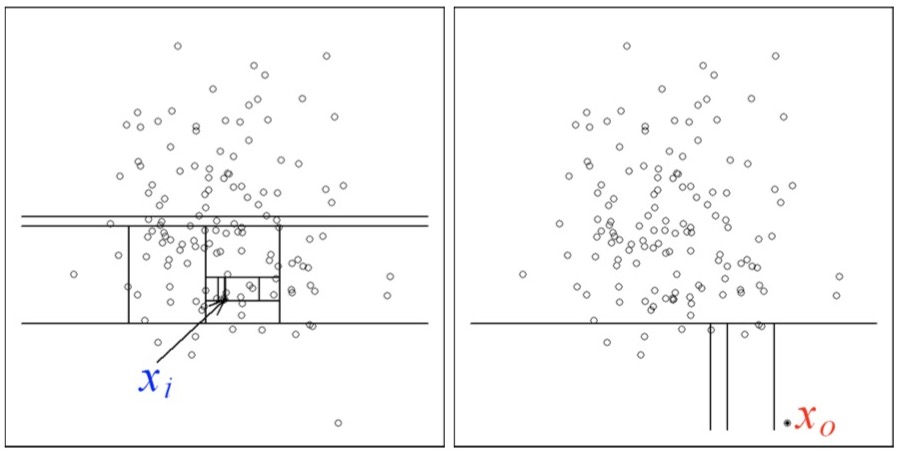
\includegraphics [scale=0.75] {iforest}
  \caption{Для изолирования точки $x_i$ требуется 12 случайных разбиений, а для аномальной точки $x_o$ -- только 4 разбиения.}
  \label{fig:iforest}
\end{figure}

\clearpage

\section{Наборы данных} \label{sec:ch2/sec5}

\noindent Для проверки сервиса были рассмотрены следующие наборы данных:
\begin{enumerate}
  \item Arrhythmia -- определение наличия аритмии по данным ЭКГ \cite{guvenir}.
  \item Breast Cancer -- определение типа опухоли молочной железы: доброкачественная или злокачественная.
  \item Glass -- идентификация типа стекла, оставленного на месте преступления.
  \item Ionosphere -- рассматриваются характеристики радаров, которые используется в анализе ионосферы: необходимо определить является радар "плохим" или "хорошим".
  \item Letter Recognition -- по описанию изображения определить присутствует ли буква из английского алфавита или нет.
  \item Mammography -- детектирование микрокальцинатов по данным маммографии.
  \item MNIST -- научиться различать изображения рукописных цифр 6 и 0.
  \item Satellite -- определение типа почвы по спутниковым снимкам.
\end{enumerate}
В качестве источника этих данных выступает библиотека ODDS \cite{odds}.

\begin{table} [htbp]
	\centering
	\caption{Статистика по данным из рассматриваемых наборов данных.}\label{tab:stats}%
	\begin{tabular}{lrrr}
		\toprule
		     Датасет & Кол-во объектов & Размерность &  Процент аномалий \\
		\midrule
		  arrhythmia &      452 &         274 &      14.60 \\
		     breastw &      683 &           9 &      34.99 \\
		       glass &      214 &           9 &       4.21 \\
		  ionosphere &      351 &          33 &      35.90 \\
		      letter &     1600 &          32 &       6.25 \\
		 mammography &    11183 &           6 &       2.33 \\
		       mnist &     7603 &         100 &       9.21 \\
		   satellite &     6435 &          36 &      31.64 \\
		\bottomrule
		\hline
	\end{tabular}
\end{table}

\noindent В таблице~\ref{tab:stats} приведено сравнение наборов данных, которые использовались для оценки качества алгоритмов. Также был рассчитан процент аномалий для каждого из наборов.

\clearpage

\section{Визуализация данных}

Рассматриваемые наборы данных имеют высокую размерность, что означает невозможность представления данных на плоскости без применения каких-либо методов. Поэтому необходимо понизить размерность до двух, чтобы отобразить объекты каждого из наборов данных на плоскости -- для этого использовался алгоритм понижения размерности t-SNE\footnote{\url{https://scikit-learn.org/stable/modules/generated/sklearn.manifold.TSNE.html}}. На~рисунке~\ref{fig:2d_comparison} представлены данные после понижения размерности.

\begin{figure}[ht]
  \centering
  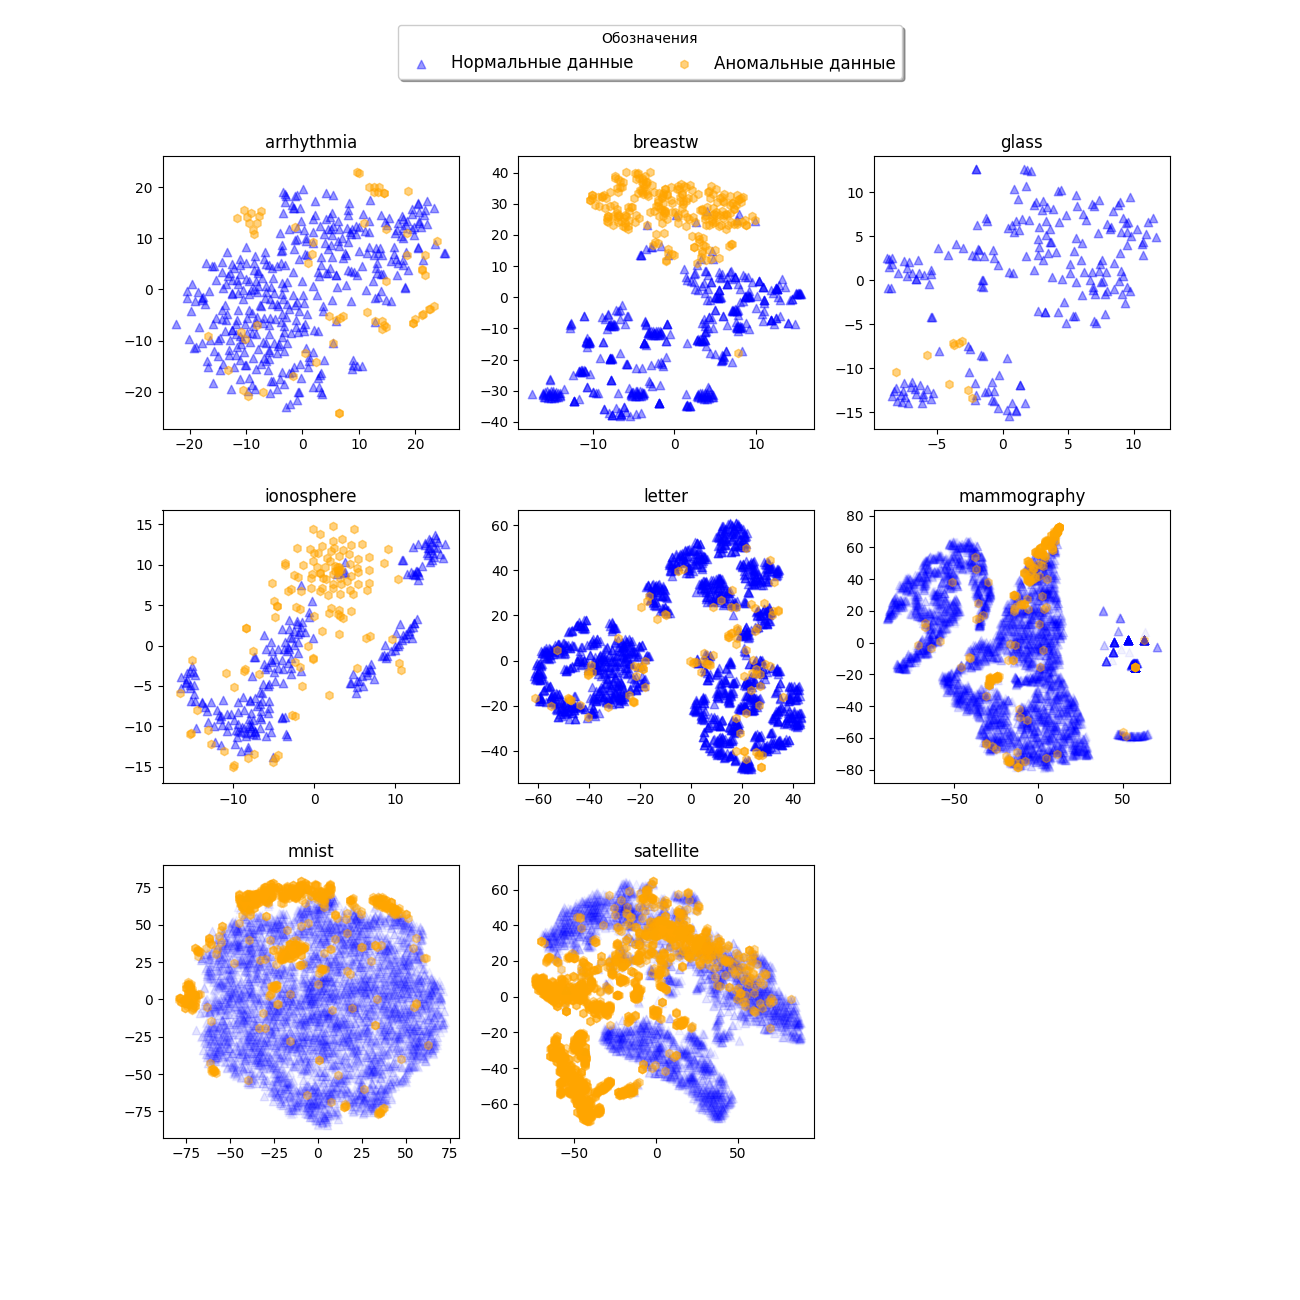
\includegraphics[width=\textwidth, height=\textheight, keepaspectratio] {2d_comparison}
  \caption{Рассматриваемые наборы данных после применения алгоритма понижения размерности t-SNE.}
  \label{fig:2d_comparison}
\end{figure}

\clearpage

\section{Эксперименты}

После подготовки данных на них были обучены и протестированы рассматриваемые алгоритмы. Набор данных разбивался на две непересекающиеся части: на первой части алгоритм обучался, а на второй -- проверялось качество обученного алгоритма. Обычно, разделение происходит в соотношении 75\% и 25\% соответственно. Так снижается вероятность переобучения на данных, что позволяет избежать ухудшения обобщающей способности алгоритмов.

В~таблице~\ref{tab:rocs} представлены результаты экспериментов оценки качества рассматриваемых алгоритмов на каждом наборе данных. Жирным шрифтом выделены наилучшие алгоритмы для каждого набора данных, которые продемонстрировали самую высокую оценку по методу ROC-AUC.

\begin{table} [htbp]
	\centering
	\caption{Значения ROC для рассматриваемых алгоритмов на данных.}\label{tab:rocs}%
	\begin{tabular}{lrrrrrr}
		\toprule
		     Датасет &   KNN &   PCA &  OCSVM &   LOF &  HBOS &  IFOREST \\
		\midrule   
   		arrhythmia &  0.7555 &  0.7794 &  0.7825 &  0.7672 &  0.7831 &   \textbf{0.7849} \\
     breastw &  \textbf{0.9908} &  0.9608 &  0.9649 &  0.4574 &  0.9764 &   0.9872 \\
       glass &  \textbf{0.8558} &  0.7308 &  0.8077 &  0.6538 &  0.7500 &   0.7212 \\
  ionosphere &  \textbf{0.9460} &  0.8115 &  0.8684 &  0.9023 &  0.6190 &   0.8632 \\
      letter &  \textbf{0.8660} &  0.5119 &  0.5985 &  0.8530 &  0.5532 &   0.5770 \\
 mammography &  0.8346 &  \textbf{0.9039} &  0.8911 &  0.6806 &  0.8506 &   0.8680 \\
       mnist &  0.8322 &  \textbf{0.8493} &  0.8487 &  0.6727 &  0.5607 &   0.7942 \\
   satellite &  0.6795 &  0.5601 &  0.6274 &  0.5567 &  \textbf{0.7464} &   0.7008 \\
		\bottomrule
		\hline
	\end{tabular}
\end{table}

\begin{figure}[ht]
  \centering
  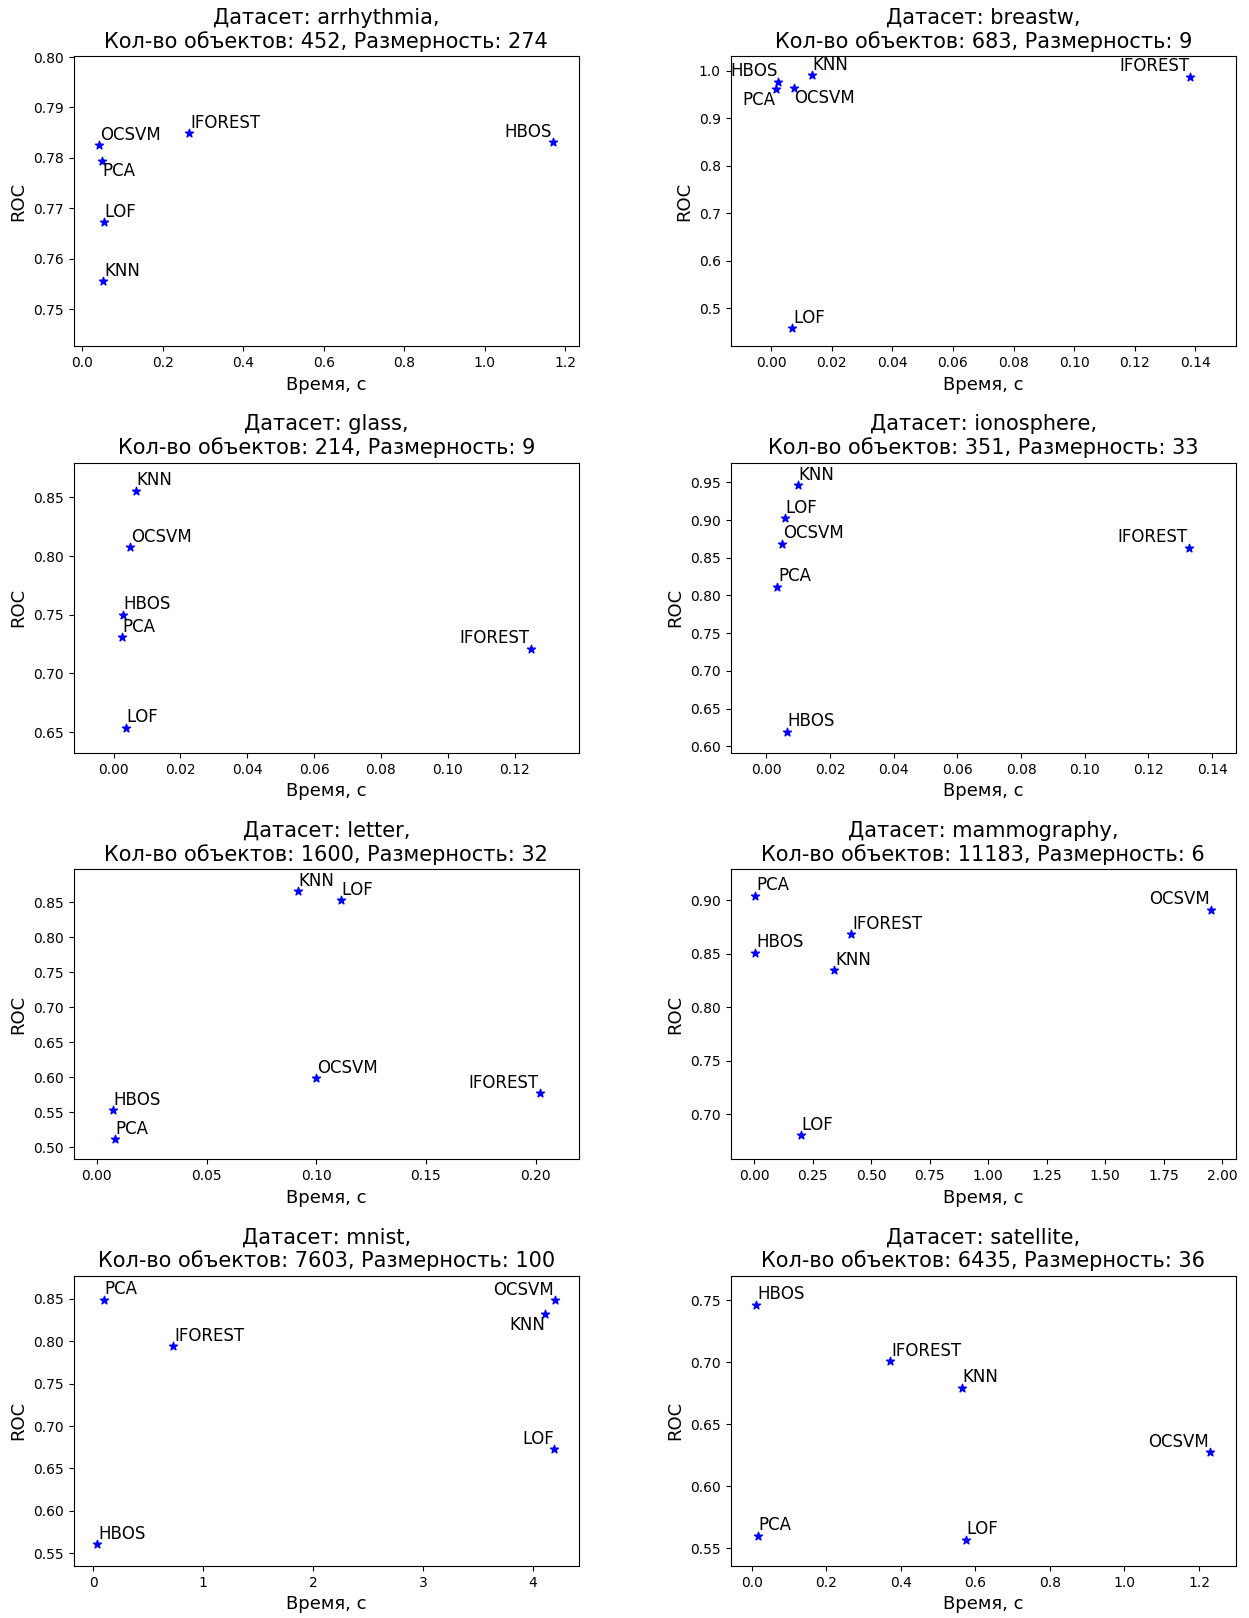
\includegraphics[width=\textwidth, height=\textheight, keepaspectratio] {roc_vs_time}
  \caption{Эффективность алгоритмов на разных наборах данных.}
  \label{fig:roc_vs_time}
\end{figure}

На графиках, которые изображены на рисунке~\ref{fig:roc_vs_time}, показана эффективность работы рассматриваемых алгоритмов на каждом наборе данных. При построении графиков использовалась библиотека adjustText\footnote{\url{https://github.com/Phlya/adjustText/}}.

\begin{figure}[ht]
  \centering
  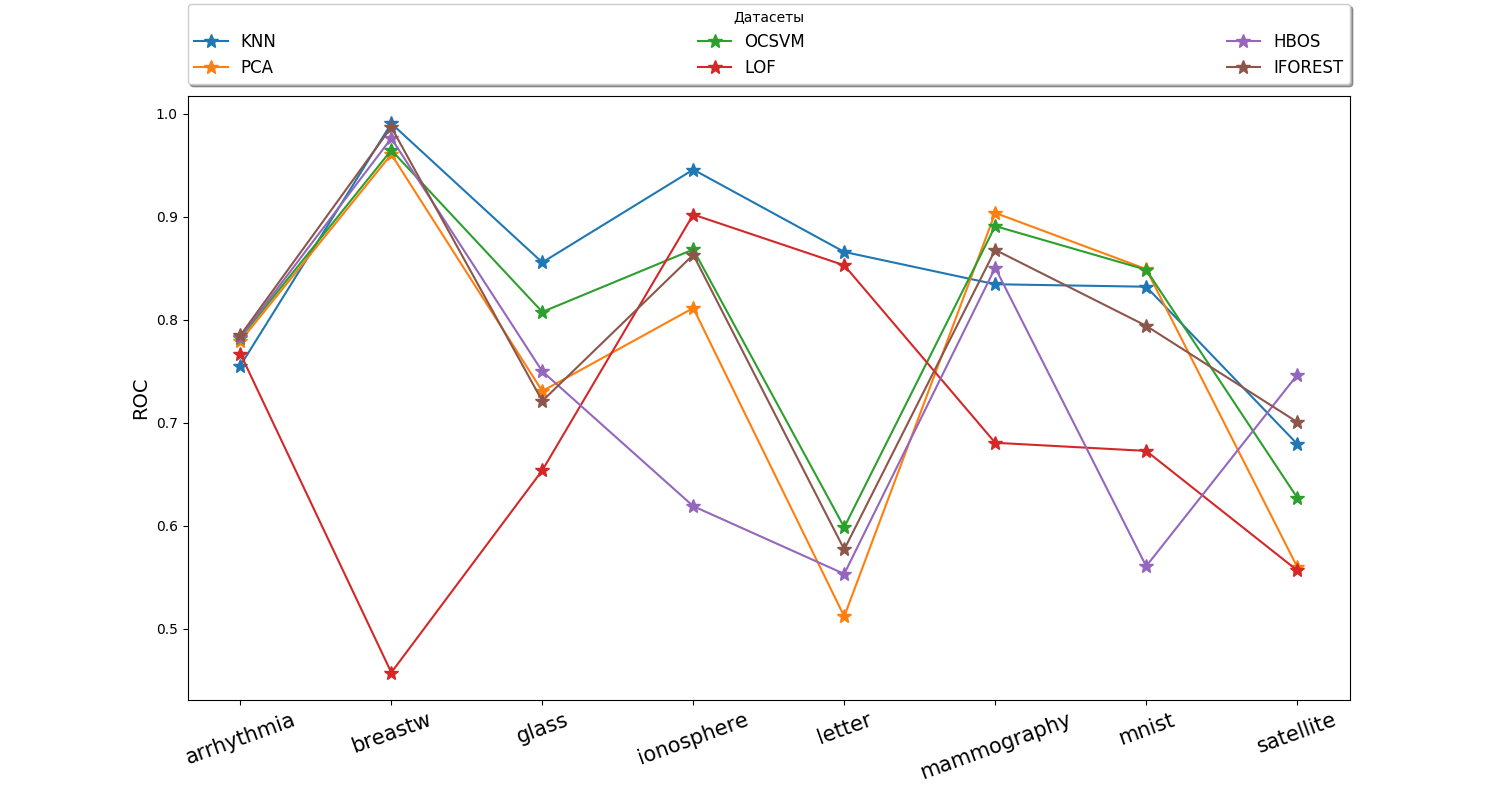
\includegraphics[width=\textwidth, height=\textheight, keepaspectratio] {roc_vs_dataset}
  \caption{Качество алгоритмов в зависимости от набора данных.}
  \label{fig:roc_vs_dataset}
\end{figure}

Согласно~таблице~\ref{tab:rocs} наилучшее качество показал алгоритм k-NN на наборе данных breastw (Breast Cancer). На~рисунке~\ref{fig:d_breastw}) продемонстрирован результат работы обученного алгоритма на этом датасете после понижения размерности с помощью метода t-SNE.

\begin{figure}[ht]
  \centering
  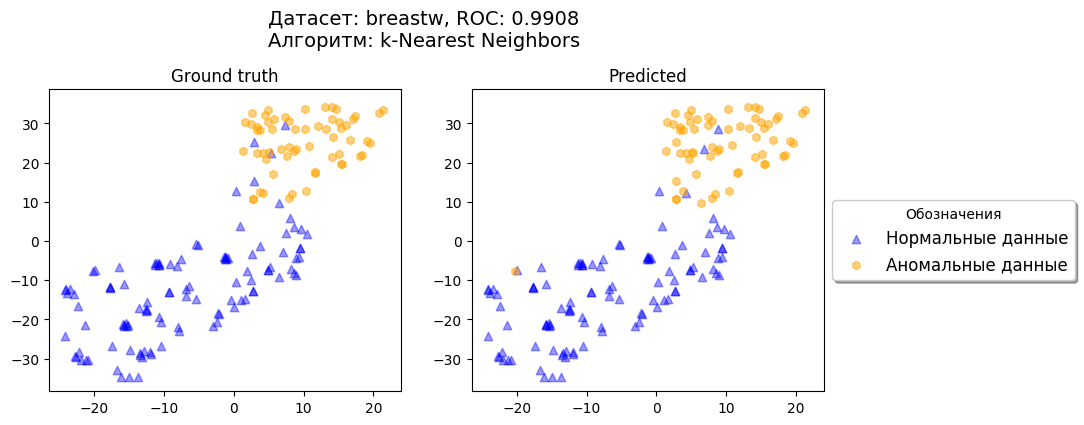
\includegraphics[width=\textwidth, height=\textheight, keepaspectratio] {d_breastw}
  \caption{Датасет Breast Cancer.}
  \label{fig:d_breastw}
\end{figure}

\clearpage
